\documentclass[epsfig,10pt,fullpage]{article}

\newcommand{\LabNum}{6}
\newcommand{\CommonDocsPath}{../../../../common/docs}
\input{\CommonDocsPath/preamble.tex}

\begin{document}
~\\
\centerline{\huge Laboratory Exercise 6}
~\\
\centerline{\large Using C Code with the Nios\textsuperscript{\textregistered} V Processor}
~\\

This is an exercise in using C code with the Nios\textsuperscript{\textregistered}~V processor.
We assume that you are using the {\it DE1-SoC Computer System with Nios~V},
which is described as part of the \texttt{Computer Organization} course on the website
{\href{https://www.fpgacademy.org/courses.html} {FPGAcademy.org}}.
A good approach is to first implement your C code for each part of this exercise by 
using the {\it CPUlator} simulator, and then to implement your solution in a hardware board,
if available.  If a hardware system other than the DE1-SoC Computer is being used, then 
some parts of this exercise may need to be modified to suit the features of your board. 

~\\
To do this exercise you need to have a good understanding of the use of arrays and 
pointers in C code. You also need to know how to use various I/O ports in the
DE1-SoC Computer System, including the {\it SW} slide switches, {\it KEY} pushbuttons,
{\it LEDR} lights, 7-segment displays, and the Nios~V Machine Timer. 
These I/O ports are described in the documentation for the 
DE1-SoC Computer System and are also discussed in Laboratory Exercise 3.

\section*{Part I}
\addcontentsline{toc}{1}{Part I}
In Laboratory Exercise 1, Part II, you were given a program in the Nios~V assembly language 
that finds the largest number in a list of 32-bit integers that is stored in the memory. 
This code is reproduced in Figure~\ref{fig:code}. For this exercise you are to write a 
C-language program that implements this task.

~\\
Perform the following steps.

\begin{enumerate}
\item
Write your C code in a file called {\it part1.c}.  You should use the {\it printf}
library function to display the result produced by the program. To use the {\it printf} function 
you have to include the {\it stdio.h} library header file in your C program by using the statement

\begin{lstlisting}[language=C]
#include <stdio.h>
\end{lstlisting}

To include a list of data words in the C program, you can declare them as an array using
a statement such as

\begin{lstlisting}[language=C]
int LIST[8] = {7, 4, 5, 3, 6, 1, 8, 2}; // number of elements, element 1,
                                        // element 2, ...
\end{lstlisting}

\item
Compile, debug, and test your C code.  When you run your program, the results produced by the
{\it printf} function should appear in the {\it Terminal} window.
Examine the assembly language code produced by the C compiler and compare it to the code 
shown in Figure~\ref{fig:code}. Note that the assembly code that implements your C
statements will not start at the address 0 in memory. Instead, at address 0 there will be 
a sequence of instructions known as the {\it C Startup Code}. To find the assembly
instructions that correspond to your C code when using the {\it CPUlator} search
in the \texttt{Disassembly} tab for the label {\it main}. If using the {\it GDB} tools,
then execute the command \texttt{disassemble main} in the {\it GDB Client}.
\end{enumerate}

\begin{figure}[H]
\begin{center}
\lstinputlisting[style=defaultNiosVStyle]{../design_files/part2.s}
\end{center}
\caption{Assembly-language program that finds the largest number.}
\label{fig:code}
\end{figure}

\section*{Part II}
\addcontentsline{toc}{2}{Part II}
Using the {\it printf} function results in a fairly large number of assembly-language instructions,
because the standard library routines are quite complex. Modify your program to display the 
result on the red lights {\it LEDR}, instead of using the {\it printf} statement. 

~\\
Put your code in a file named {\it part2.c}.
Compile, download, and run this program. Observe the difference in the size of the
machine code for this program as compared to the one from Part I.

\section*{Part III}
\addcontentsline{toc}{3}{Part III}
In Part I of Laboratory Exercise 2 you were given a program that uses shift and AND operations
to find the longest string of 1's in a word of data. The program is reproduced in
Figure~\ref{fig:shiftAND}.  In Part II of Exercise 2 you were asked to extend
this program so that it processed a list of data words, rather than just one word.
Finally, in Part III you were asked to find the longest string of 0's in any word in the
list, and in Part IV the longest string of alternating 1's and 0's.

~\\
For this part of the exercise you are to implement all of the parts of Laboratory Exercise 2 
using C code. Your program should find the longest sequence of 1's, 0's, and alternating 0's and
1's in a list of data words.

\begin{figure}[H]
\begin{center}
\lstinputlisting[style=defaultNiosVStyle]{../design_files/part3.s}
\end{center}
\caption{Assembly-language program that counts consecutive ones.}
\label{fig:shiftAND}
\end{figure}

To include the list of data words in your C program, you can declare them as an array using
a statement such as

\begin{lstlisting}[language=C]
int TEST_NUM[ ] = {0x0000e000, 0x3fabedef, 0x00000001, 0x00000002, 0x75a5a5a5,
                   0x01ffC000, 0x03ffC000, 0x55555555, 0x77777777, 0x08888888,
                   0x00000000};
\end{lstlisting}


Display the count for the longest string of 1's on 7-segment displays \red{{\it HEX1-0}}, 
for the longest string of 0's on \red{{\it HEX3-3}}, and for alternating 1's and 0's 
on \red{{\it HEX5-4}}.  All of your results are to be displayed as decimal (base 10)
numbers.

~\\
Create a file called {\it part3.c} for your code, and then compile, debug and test it. 
Using the ten words of test data shown above, the correct
result that should appear on the \red{{\it HEX5-0}} displays is \red{\sf 32 31 12}.

\section*{Part IV}
\addcontentsline{toc}{4}{Part IV}
In Exercise 3 you learned how to use the Nios~V Machine Timer with polled-I/O 
to implement an exact delay.  In this part of the exercise you are to use polled-I/O with
the Nios~V Machine Timer with C code. 

~\\
In Exercise 5 you were asked to implement a real-time clock.
The clock time was shown on the \red{{\it HEX3-0}} seven-segment displays in the 
format \red{SS}:\red{DD}, with \red{\it SS} representing seconds and \red{\it DD} 
representing hundredths of a second. 
The clock could be stopped/run by pressing one of the {\it KEY} pushbuttons, and
time was measured in intervals of 0.01 seconds by using the Nios~V Machine Timer.

~\\
In this part of the exercise you are to implement a real-time clock using C code. 
Display the clock time on the 7-segment displays \red{{\it HEX5-0}}
in the format \red{MM}:\red{SS}:\red{DD}, where 
where \red{\it MM} are minutes, \red{\it SS} are seconds, and \red{\it DD} are hundredths of 
a second.  Measure time intervals of 0.01 seconds in your program by using the 
Nios~V Machine Timer.  Unlike Exercise 5, where you used interrupt-driven I/O with the timer, in
this exercise you are to use polled-I/O with the Machine Timer to wait for each 0.01
seconds. You should be able to stop/run the clock by pressing any {\it KEY} pushbutton.
When the clock reaches \red{59}:\red{59}:\red{99}, it should wrap around to
\red{00}:\red{00}:\red{00}.

~\\
Create a file called {\it part4.c} for your C code. Compile, debug, and test your program. 
An outline of how your code could be structured is given in Figure~\ref{fig:outlineIV}.

\begin{figure}[H]
\begin{center}
\begin{minipage}[h]{15.5 cm}
\lstinputlisting[language=C]{../design_files/part4.c}
\caption{An outline of the code for Part IV.}
\label{fig:outlineIV}
\end{minipage}
\end{center}
\end{figure}

\section*{Part V}
\addcontentsline{toc}{5}{Part V}
Write a C program that scroll a message, such as \red{\sf dE1-SoC},
in the right-to-left direction across the 7-segment displays.
An example of the scrolling behaviour is given in Table~\ref{tab:scrolling}.
You should scroll the display at a rate that is visually appealing. You should be 
able to stop/run the scrolling
message by pressing the {\it KEY} pushbuttons.

~\\
Note that scrolling a message across the 7-segment displays is similar in nature to the 
task of implementing a real-time clock, from Part IV. You should be able to reuse most of 
your code from Part IV. But instead of updating the clock each time the Machine Timer
expires, you need to update the scrolling message.  

~\\
An example of how you might declare your message that is to be scrolled is shown below:
~\\
\begin{lstlisting}[language=C, escapechar=|]
char message[] = "|\red{\sf {dE1-SoC~~~~~~dE1-S}}|";  // the scrolling message
\end{lstlisting}

\newpage
\begin{table}[H]
\begin{minipage}[t]{12.5 cm}
\begin{center}
\begin{tabular}{c|cccccc}
Time slot & \multicolumn{6}{c}{Display} \\
\hline
{\rule[0mm]{0mm}{5mm}0} &\red{d}&\red{E}&\red{1}&\red{-}&\red{S}&\red{o} \\ 
1 &\red{E}&\red{1}&\red{-}&\red{S}&\red{o}&\red{C} \\
2 &\red{1}&\red{-}&\red{S}&\red{o}&\red{C}& \\
3 &\red{-}&\red{S}&\red{o}&\red{C}& & \\
4 &\red{S}&\red{o}&\red{C}& & &\\
5 &\red{o}&\red{C}& & & &\\
6 &\red{C}& & & & &\\
7 & & & & & &\\
8 & & & & & &\red{d}\\
9 & & & & &\red{d}&\red{E}\\
10 & & & &\red{d}&\red{E}&\red{1}\\
$\ldots$ & & &$\ldots$ & &\\
\end{tabular}
\caption{Scrolling the message \red{\sf dE1-SoC} on \red{{\it HEX5-0}}.}
\label{tab:scrolling}
\end{center}
\end{minipage}
\end{table}

~\\
You might want to make use of a function like the one shown below for translating the letters
in your message to 7-segment display codes:
~\\
\begin{lstlisting}[language=C]
char display(char c) {
	char seg7_code = 0;
	switch (c) {
		case 'd': seg7_code = 0b01011110; break;
		case 'E': seg7_code = 0b01111001; break;
		case '1': seg7_code = 0b00000110; break;
		case '-': seg7_code = 0b01000000; break;
		case 'S': seg7_code = 0b01101101; break;
		case 'o': seg7_code = 0b01011100; break;
		case 'C': seg7_code = 0b00111001; break;
		case ' ': seg7_code = 0b00000000; break;
	}
	return seg7_code;
}
\end{lstlisting}

Put your code in file called {\it part5.c}, compile, debug, and test it.

\section*{Part VI}
\addcontentsline{toc}{5}{Part V}
The purpose of this part of the exercise is to gain experience in using a different timer,
other than the Nios~V Machine Timer, in the DE1-SoC Computer. Modify your solution from
Part V so that instead of the Machine Timer you use polled-I/O with the {\it Interval Timer}. 

~\\
The Interval Timer is implemented in the FPGA in the DE1-SoC Computer. This timer can be 
loaded with an initial value, and then counts down to zero at a 100-MHz clock rate. 
The programming interface for the timer includes six 16-bit registers, as illustrated in 
Figure~\ref{fig:intervaltimer}.

\begin{figure}[H]
	\begin{center}
	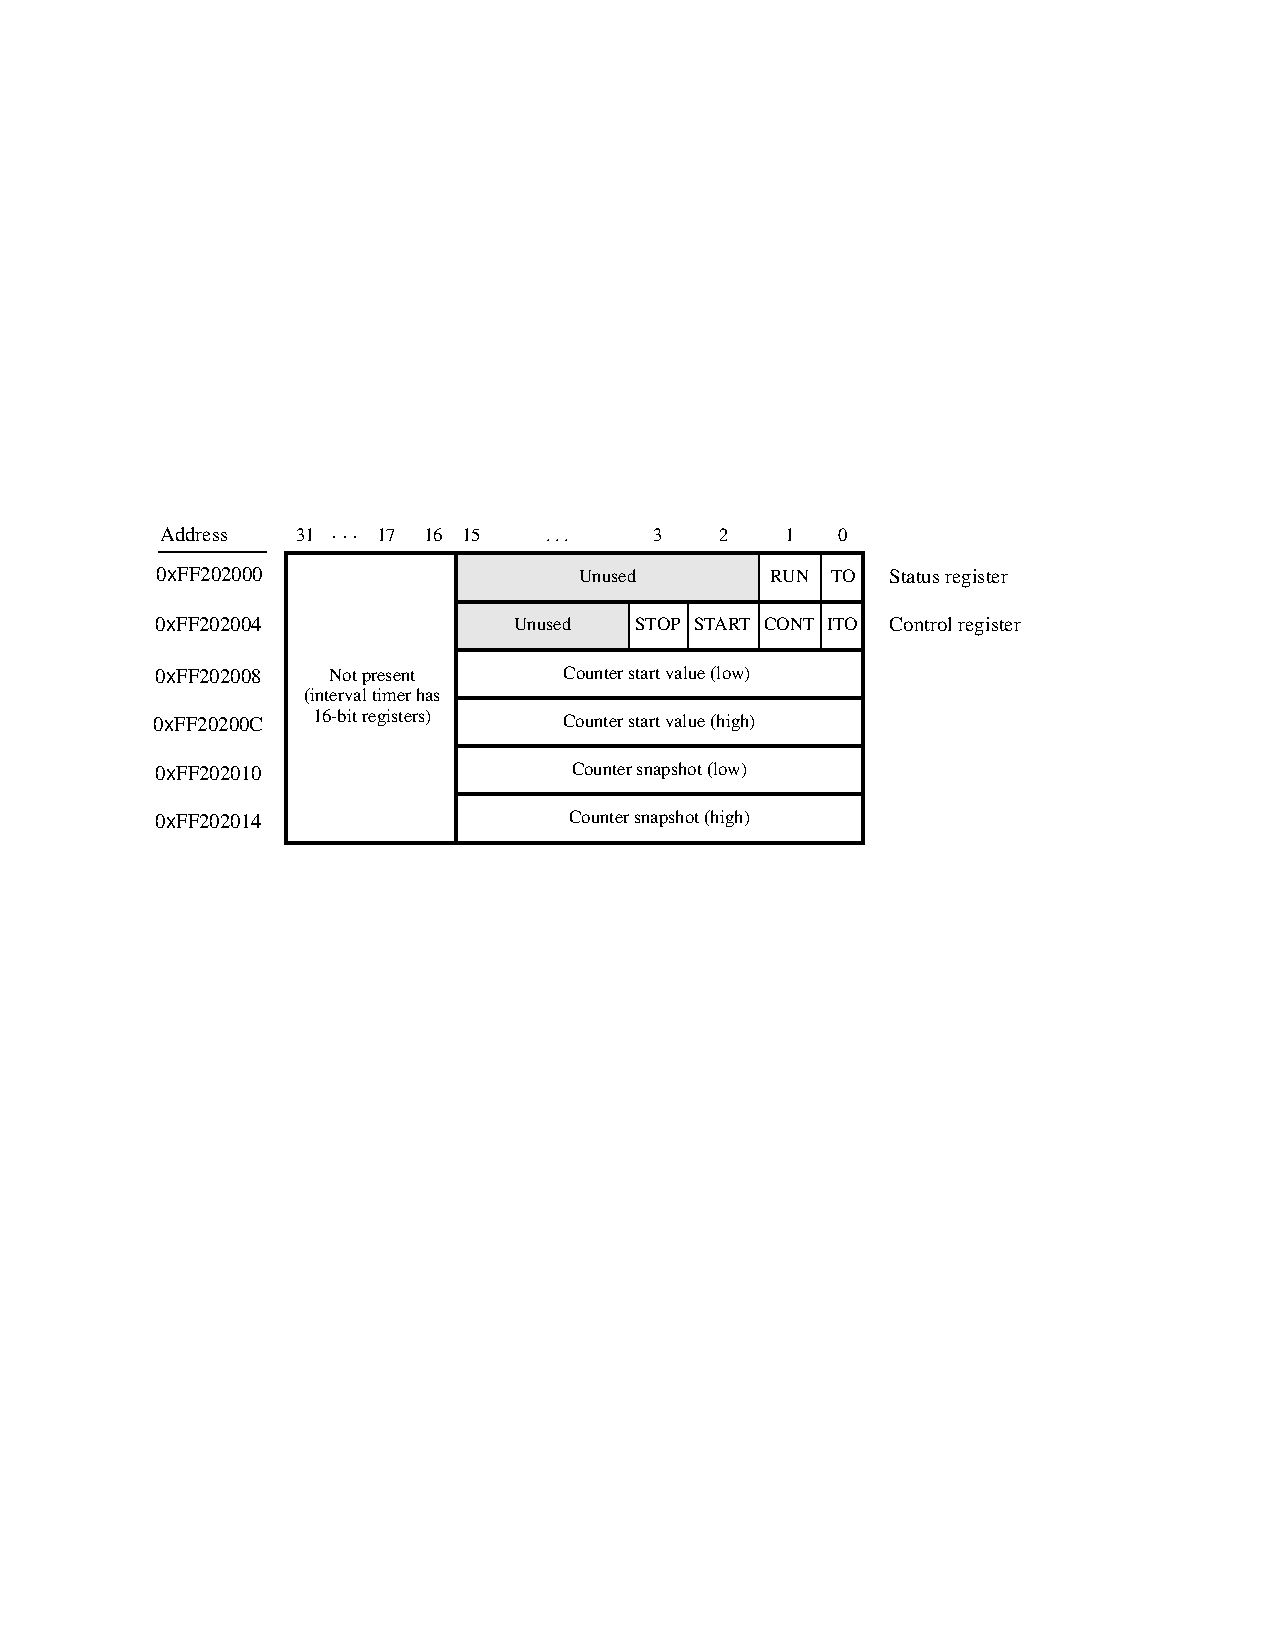
\includegraphics[scale=1]{figures/figuretimer.pdf}
	\end{center}
	\caption{The Interval Timer registers.}
\label{fig:intervaltimer}
\end{figure}

~\\
The {\it TO} bit in the {\it Status} register provides a timeout signal which is set to 1 
by the timer when it has reached a count value of zero.  
You should poll this bit in your program to cause the Nios~V processor 
to wait for the timer.  The {\it TO} bit can be reset by writing a 0 into it.  

~\\
The {\it CONT} bit affects the continuous operation of the timer.  When the timer reaches
a count value of zero it automatically reloads the specified starting count value. If 
{\it CONT} is set to 1, then the timer will continue counting down automatically.
But if {\it CONT} $=0$, then the timer will stop after it has reached a count value of 0. 
The ({\it START}/{\it STOP}) bits can be used to commence/suspend the operation of the 
timer by writing a 1 into the respective bit.

~\\
The two 16-bit {\it Counter start value} registers are used to set the timeout for the
Interval Timer. Set up the timer so that it provides the 0.01 second timeouts that are
needed for the real-time clock. 

~\\
Put your code in a file called {\it part6.c}.
Reuse most of your code from Part V, changing only the parts of the code that pertain to
the timer.  Compile, debug, and test your solution.

\input{\CommonDocsPath/copyright.tex}
\end{document}
